\begin{surferPage}{Двострука купа}
   Као што је објашњено у уводу, површ се назива 
    \emph{не-сингуларном} или глатком ако не поседује врх 
    (такве тачке се називају сингуларитетима).
    На пример, сфера или торус (слика у средини и лево):
    \begin{center}
      \begin{tabular}{@{}c@{}c@{}c@{}c@{}}
        \begin{tabular}{@{}c}
          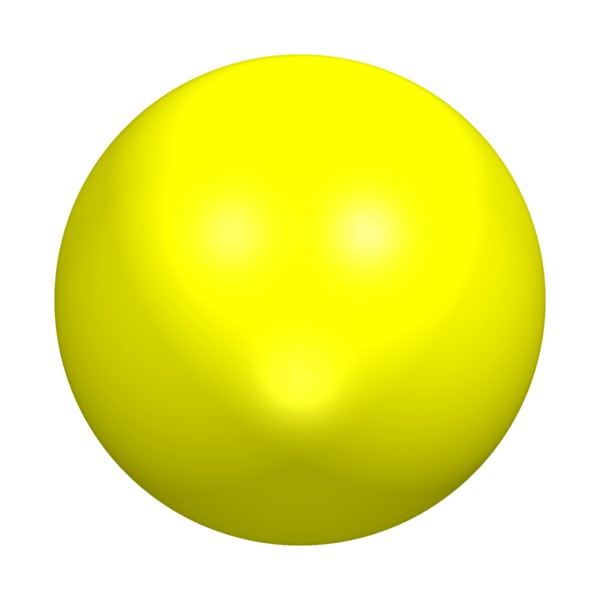
\includegraphics[width=1.4cm]{./../../common/images/kugel}
        \end{tabular}
        &
        \begin{tabular}{@{}c}
          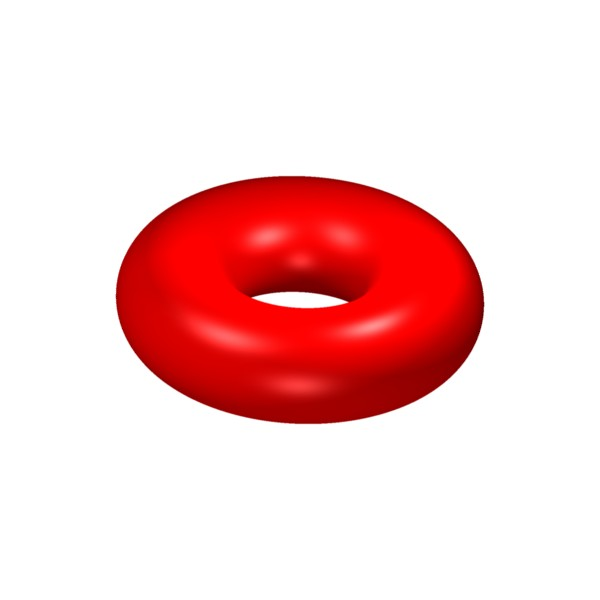
\includegraphics[width=1.4cm]{./../../common/images/torus}
        \end{tabular}
        &
        \begin{tabular}{c@{}}
          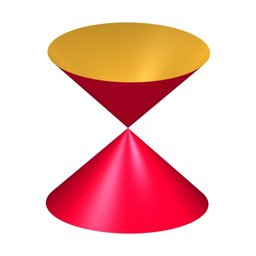
\includegraphics[width=1.4cm]{./../../common/images/kegel}
        \end{tabular}
      \end{tabular}
    \end{center}
     Двострука купа (слика десно) је најједноставнији сингуларитет; то је једини сингуларитет који се
	 може описати једначином:
    \[x^2+y^2-z^2=0.\]
    Када се у овој једначини уместо нуле напише неки параметар а, мале вредности, 
	двострука купа се трансформише у један од два типа хиперболоида, 
	зависно од знака параметра $a$:
    \begin{center}
      \begin{tabular}{@{}c@{\ }c@{\ }c@{\ }c@{\ }c@{}}
        \begin{tabular}{@{}c@{}}
          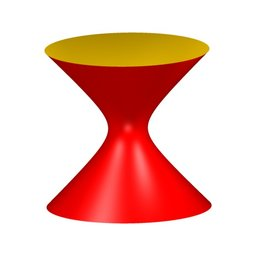
\includegraphics[width=1.2cm]{./../../common/images/A1pm_2}
        \end{tabular}
        &
        $\leftarrow$
        &
        \begin{tabular}{@{}c@{}}
          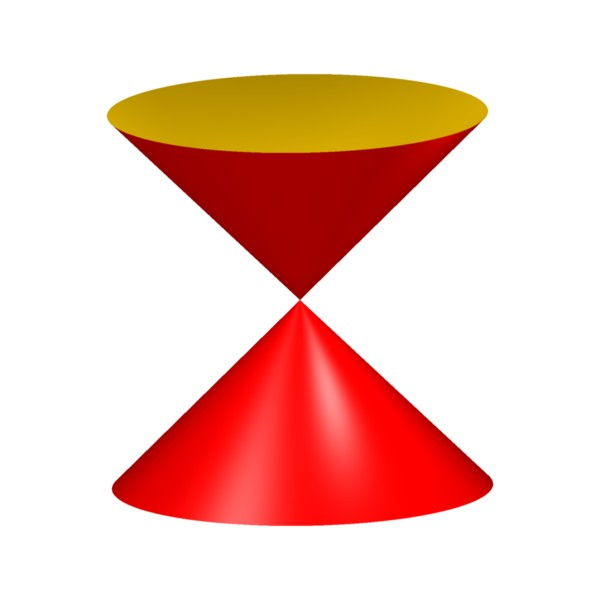
\includegraphics[width=1.2cm]{./../../common/images/A1pm_1} 
        \end{tabular}
        &
        $\rightarrow$
        &
        \begin{tabular}{@{}c@{}}
          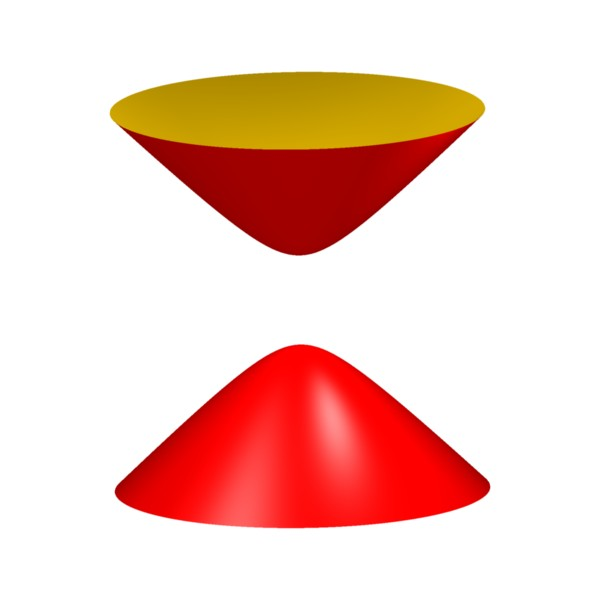
\includegraphics[width=1.2cm]{./../../common/images/A1pm_0}
        \end{tabular}
      \end{tabular}
    \end{center}
   Површ степена $2$ не може имати више од једног сингуларитета $\mu(2)=1$.
\end{surferPage}
